%----------------------------------------------------------------------------------------
% METADATA BLOCK (YAML)  — see inbox/README.md for every field
%----------------------------------------------------------------------------------------
% uid: ""
% school: "lycee"
% level: "3eme"
% section: "Mathématiques"
% chapter: "Produit scalaire dans le plan"
% title: "Le théorème du papillon"
% difficulty: "Moyen"
% tags: ["papillon", "cercle", "cordes", "coordonnees", "milieu"]
% provenance: "adapted"
% batch: "2026-11-20-defis-geometrie-A"
%----------------------------------------------------------------------------------------

% ---STATEMENT---
Soit $\mathcal C$ un cercle et $[PQ]$ une corde de $\mathcal C$ de milieu $M$. Par $M$ passent deux autres cordes $[AB]$ et $[CD]$ (ni l'une ni l'autre n'est la corde $[PQ]$ ni perpendiculaire à $[PQ]$). Les droites $(AD)$ et $(BC)$ coupent $(PQ)$ en $X$ et $Y$.

% alt: Cercle, corde PQ de milieu M, deux cordes AB et CD passant par M, les droites AD et BC coupent PQ en X et Y
\begin{center}
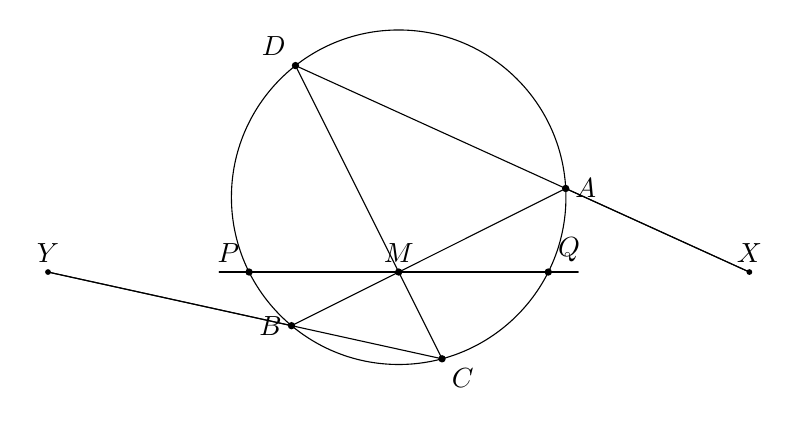
\begin{tikzpicture}[scale=0.95,line cap=round,line join=round,>=stealth]
\draw (0,1) circle (2.236);
\draw[] (-2,0) -- (2,0);
\draw[] (2.233,1.117) -- (-1.433,-0.717);
\draw[] (0.58,-1.16) -- (-1.38,2.76);
\draw[thin] (-1.38,2.76) -- (4.688,0);
\draw[thin] (2.233,1.117) -- (4.688,0);
\draw[thin] (-1.433,-0.717) -- (-4.688,0);
\draw[thin] (0.58,-1.16) -- (-4.688,0);
\draw[] (-2.4,0) -- (-2,0);
\draw[] (2,0) -- (2.4,0);
\fill(-2,0) circle (1.4pt) node[above left] {$P$};
\fill(2,0) circle (1.4pt) node[above right] {$Q$};
\fill(0,0) circle (1.4pt) node[above] {$M$};
\fill(2.233,1.117) circle (1.4pt) node[right] {$A$};
\fill(-1.433,-0.717) circle (1.4pt) node[left] {$B$};
\fill(0.58,-1.16) circle (1.4pt) node[below right] {$C$};
\fill(-1.38,2.76) circle (1.4pt) node[above left] {$D$};
\fill(4.688,0) circle (1.1pt) node[above] {$X$};
\fill(-4.688,0) circle (1.1pt) node[above] {$Y$};
\end{tikzpicture}
\end{center}

On veut montrer que \textbf{$M$ est le milieu de $[XY]$}. On rapporte le plan au repère orthonormé d'origine $M$, dont l'axe des abscisses est $(PQ)$. On pose $MP=MQ=m>0$ ; le centre $O$ de $\mathcal C$ est alors sur l'axe des ordonnées, $O(0,k)$.
\begin{enumerate}
  \item Montrer que $\mathcal C$ a pour équation $x^2+y^2-2ky-m^2=0$.
  \item Une droite $y=\lambda x$ passant par $M$ recoupe $\mathcal C$ en deux points d'abscisses $x_1$ et $x_2$. Montrer que $x_1+x_2=\dfrac{2k\lambda}{1+\lambda^2}$ et $x_1x_2=-\dfrac{m^2}{1+\lambda^2}$, puis que
  \[\dfrac1{x_1}+\dfrac1{x_2}=-\dfrac{2k\lambda}{m^2}.\]
  \item Les cordes $[AB]$ et $[CD]$ portées par $y=\lambda x$ et $y=\mu x$ ($\lambda\neq\mu$), $A$ et $B$ ont pour abscisses $x_1,x_2$ et $C$, $D$ pour abscisses $x_3,x_4$. Calculer en fonction de $\lambda$, $\mu$, $x_1$, $x_4$ l'abscisse $X$ du point d'intersection de $(AD)$ avec l'axe $(Mx)$, puis l'abscisse $Y$ de $(BC)\cap(Mx)$.
  \item Calculer $\dfrac1X+\dfrac1Y$ et conclure.
\end{enumerate}

% ---SOLUTION---
\begin{enumerate}[itemsep=14pt]
  \item $O$ est sur la médiatrice de $[PQ]$, c'est-à-dire sur l'axe des ordonnées (puisque $M$ est le milieu de $[PQ]$ et $(PQ)$ est l'axe des abscisses) : $O(0,k)$. $P(-m,0)$ est sur $\mathcal C$.

  \begin{prop}[Équation d'un cercle]
  Le cercle de centre $\Omega(x_0,y_0)$ et de rayon $\rho$ a pour équation \ib{$(x-x_0)^2+(y-y_0)^2=\rho^2$}.
  \end{prop}
  $\mathcal C$ : $x^2+(y-k)^2=R^2$. Le point $P(-m,0)$ y est : $m^2+k^2=R^2$.

  En développant : $x^2+y^2-2ky+k^2-R^2=0$, soit \ib{$x^2+y^2-2ky-m^2=0$}.

  \item On remplace $y=\lambda x$ dans l'équation :
  \[x^2+\lambda^2x^2-2k\lambda x-m^2=0\iff(1+\lambda^2)x^2-2k\lambda x-m^2=0.\]
  \begin{prop}[Somme et produit des racines]
  Pour $ax^2+bx+c=0$ de racines $x_1,x_2$ : \ib{$x_1+x_2=-\dfrac ba$} et \ib{$x_1x_2=\dfrac ca$}.
  \end{prop}
  \[x_1+x_2=\dfrac{2k\lambda}{1+\lambda^2},\qquad x_1x_2=-\dfrac{m^2}{1+\lambda^2}.\]
  Donc
  \[\dfrac1{x_1}+\dfrac1{x_2}=\dfrac{x_1+x_2}{x_1x_2}=\dfrac{2k\lambda}{1+\lambda^2}\times\left(-\dfrac{1+\lambda^2}{m^2}\right)=-\dfrac{2k\lambda}{m^2}.\]
  Cette somme est proportionnelle à la pente $\lambda$ : \textbf{$\dfrac1{x_1}+\dfrac1{x_2}=-\dfrac{2k}{m^2}\,\lambda$}.

  \item $A(x_1,\lambda x_1)$ et $D(x_4,\mu x_4)$. L'abscisse du point où la droite $(AD)$ coupe $y=0$ est
  \begin{prop}[Intersection d'une droite avec l'axe des abscisses]
  La droite passant par $U(x_U,y_U)$ et $V(x_V,y_V)$ avec $y_U\neq y_V$ coupe $y=0$ en \ib{$x=\dfrac{x_Uy_V-x_Vy_U}{y_V-y_U}$}.
  \end{prop}
  \[X=\dfrac{x_1\cdot\mu x_4-x_4\cdot\lambda x_1}{\mu x_4-\lambda x_1}=\dfrac{x_1x_4(\mu-\lambda)}{\mu x_4-\lambda x_1}.\]
  De la même façon, $B(x_2,\lambda x_2)$ et $C(x_3,\mu x_3)$ :
  \[Y=\dfrac{x_2x_3(\mu-\lambda)}{\mu x_3-\lambda x_2}.\]

  \item On passe aux inverses :
  \[\dfrac1X=\dfrac{\mu x_4-\lambda x_1}{x_1x_4(\mu-\lambda)}=\dfrac{\dfrac\mu{x_1}-\dfrac\lambda{x_4}}{\mu-\lambda},\qquad\dfrac1Y=\dfrac{\dfrac\mu{x_2}-\dfrac\lambda{x_3}}{\mu-\lambda}.\]
  On additionne :
  \[\dfrac1X+\dfrac1Y=\dfrac{\mu\left(\dfrac1{x_1}+\dfrac1{x_2}\right)-\lambda\left(\dfrac1{x_3}+\dfrac1{x_4}\right)}{\mu-\lambda}.\]
  D'après la question 2, $\dfrac1{x_1}+\dfrac1{x_2}=-\dfrac{2k\lambda}{m^2}$ (droite $y=\lambda x$) et $\dfrac1{x_3}+\dfrac1{x_4}=-\dfrac{2k\mu}{m^2}$ (droite $y=\mu x$). Donc
  \[\dfrac1X+\dfrac1Y=\dfrac{-\dfrac{2k\lambda\mu}{m^2}+\dfrac{2k\lambda\mu}{m^2}}{\mu-\lambda}=0.\]
  Donc $Y=-X$ (ni $X$ ni $Y$ n'est nul : $X=0$ signifierait que $A$, $M$, $D$ sont alignés, c'est-à-dire $D\in(AB)$).

  $X$ et $Y$ sont opposés : \ib{$M$ est le milieu de $[XY]$}. $\blacksquare$
\end{enumerate}

\textbf{Remarque.} Il existe d'autres preuves du théorème du papillon (trigonométrique, par les aires, projective) ; celle-ci est purement algébrique.

\textbf{Idée :} la quantité $\dfrac1{x_1}+\dfrac1{x_2}$ ne dépend de la corde que par sa pente, grâce au fait que $M$ est le milieu de $[PQ]$ ; on la retrouve, avec les mêmes coefficients, pour les deux cordes, et elle s'annule dans la combinaison $\mu(\cdots)-\lambda(\cdots)$.

\textbf{Piège :} bien appareiller $A$ avec $D$ et $B$ avec $C$ pour $X$ et $Y$ ; l'identité reste vraie si on échange les noms de $C$ et $D$, car seules les sommes $\dfrac1{x_1}+\dfrac1{x_2}$ et $\dfrac1{x_3}+\dfrac1{x_4}$ interviennent.
